\documentclass{article}
\usepackage{graphicx} % Required for inserting images

\usepackage{tikz}
\usetikzlibrary{shapes.geometric, arrows}

% Presets, change here 
\tikzstyle{blue} = [rectangle, rounded corners, minimum width=3cm, minimum height=1cm,text centered, draw=black, fill=blue!30]
\tikzstyle{red} = [rectangle, rounded corners, minimum width=3cm, minimum height=1cm,text centered, draw=black, fill=red!30]
\tikzstyle{gold} = [rectangle, rounded corners, minimum width=3cm, minimum height=1cm,text centered, draw=black, fill=yellow!30]
\tikzstyle{goldenRod} = [rectangle, rounded corners, minimum width=3cm, minimum height=1cm,text centered, draw=black, fill=yellow!85]

\tikzstyle{arrow} = [thick,->,>=stealth]



\begin{document}
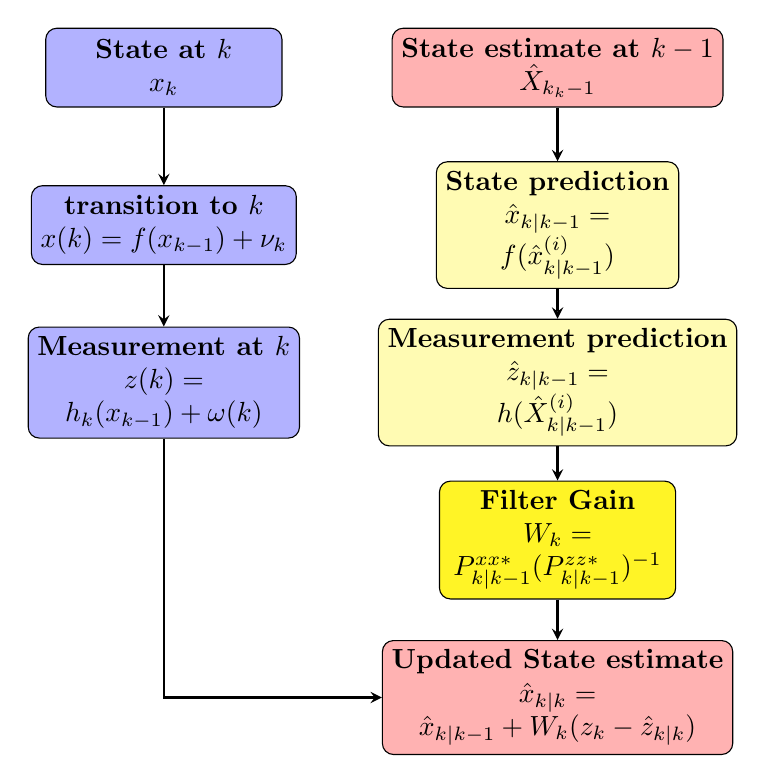
\begin{tikzpicture}[node distance=2cm]


%  Don't touch this          this is nickname     see presets above               The actual Text
% \node[draw, align=center]   (stateAT)          [blue]                      {\textbf{State at $t_k$} \\ $x(k)$};


% Column 1 - Evolution of the System (true state)
\node[draw, align=center] (stateAT) [blue] {\textbf{State at $k$} \\ $x_k$};
\node[draw, align=center] (transTO) [blue, below of=stateAT] {\textbf{transition to $k$} \\ $x(k) = f(x_{k-1})+\nu_k$};
\node[draw, align=center] (measAT) [blue, below of=transTO] {\textbf{Measurement at $k$} \\ $z(k) = $\\$h_{k}(x_{k-1}) + \omega(k)$};

% Column 2 - Estimation of the State
\node[draw, align=center] (stateEST) [red, right of=stateAT, xshift=3cm] {\textbf{State estimate at $k-1$} \\ $\hat{X}_{k_k-1}$};
\node[draw, align=center] (statePRED) [gold, below of=stateEST] {\textbf{State prediction} \\ $\hat{x}_{k|k-1} =$ \\ $f(\hat{x}_{k|k-1}^{(i)})$};
\node[draw, align=center] (measPRED) [gold, below of=statePRED] {\textbf{Measurement prediction} \\ $\hat{z}_{k|k-1}=$ \\ $h(\hat{X}_{k|k-1}^{(i)})$ };


\node[draw, align=center] (filterG) [goldenRod, below of=measPRED] {\textbf{Filter Gain} \\ $W_k=$ \\   $P^{xx*}_{k|k-1} (P^{zz*}_{k|k-1})^{-1}$};

\node[draw, align=center] (updateEST) [red, below of=filterG] {\textbf{Updated State estimate} \\ $\hat{x}_{k|k} =$ \\ $\hat{x}_{k|k-1}+W_k(z_k-\hat{z}_{k|k})$};


%  Don't touch this             From here        either --, |-, or -|                 to here
% \draw [arrow]             (stateAT)               --                               (transTO);

% Column 1 - Arrows
\draw [arrow] (stateAT) -- (transTO);
\draw [arrow] (transTO) -- (measAT);
\draw [arrow] (measAT) |- (updateEST);

% Column 2 - Arrows
\draw [arrow] (stateEST) -- (statePRED);
\draw [arrow] (statePRED) -- (measPRED);
\draw [arrow] (measPRED) -- (filterG);
\draw [arrow] (filterG) -- (updateEST);

\end{tikzpicture}




\end{document}